
\begin{frame}
	\frametitle{About Matplotlib}

    \begin{itemize}
    \item Python-based, open-source plotting library
    \item Available for all Python installations for different operating systems
    \item Uses data structures from other Python libraries like NumPy
    \item Integrates well with Python scientific libraries (NumPy, SciPy,...)
    \item Together with these libraries provides Matlab-like functionality 
    \item Access to Python file processing functions for convenient, cross-platform data handling 
    \item Can by used interactively in environments like Jupyter or in batch mode
    \item Plots can be saved in various file formats including PNG bitmap and PDF vector graphics
    \end{itemize}

\end{frame}

\begin{frame}
	\frametitle{Installation}
    \begin{itemize}
      \item For Windows and macOS:		
      \item Anaconda Python: https://www.anaconda.com/products/individual
			\item If not included: \kommandozeile{conda install -c conda-forge matplotlib}      
      \item Linux variants:
      \item Use package manager to install python
			\item Use pip to install matplotlib: \kommandozeile{pip install -U matplotlib}
			\item Use Jupyter online to try it online: https://jupyter.org/try
			\item Anaconda install Jupyter Windows/macOS: \kommandozeile{conda install ipython jupyter}
			\item Pip install Jupyter: \kommandozeile{pip install --upgrade ipython jupyter}
    \end{itemize}
\end{frame}

\begin{frame}
    \begin{center}
      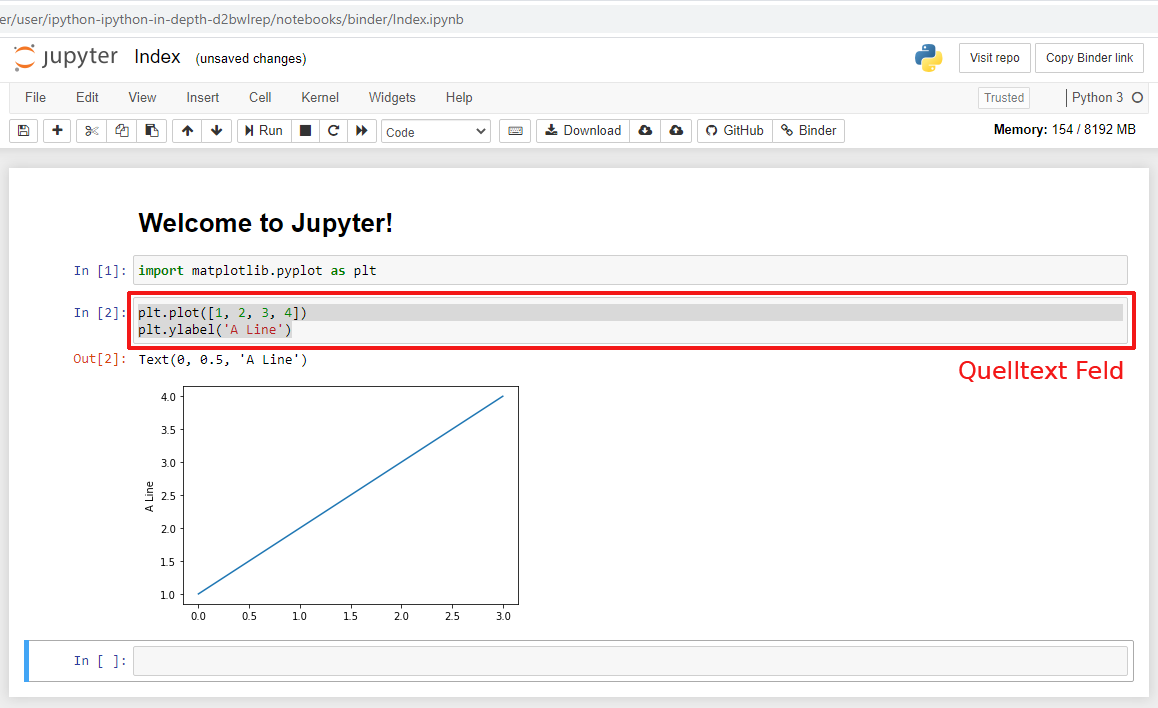
\includegraphics[width=0.9\textwidth]{screenshots/jupyter-1.png}
    \end{center}		
\end{frame}

\begin{frame}
	\frametitle{Start a Juypter Notebook}
    \begin{itemize}
      \item Command line, Terminal or CMD: \kommandozeile{jupyter notebook}
      \item Runs in browser window
			\item In Visual Studio Code with Python Extension: 
			\item \keyword{STRG + SHIFT + P->Jupyter: Create New Blank Jupyter Notebook} 			
    \end{itemize}
    \begin{center}
      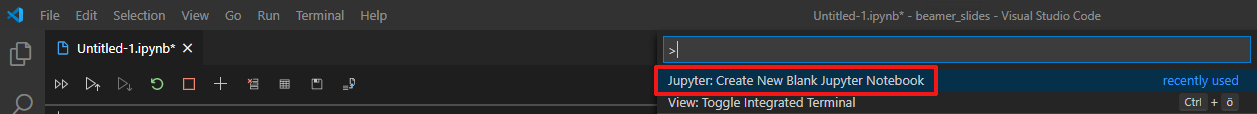
\includegraphics[width=1.0\textwidth]{screenshots/vsc-2.png}
    \end{center}				
\end{frame}

\begin{frame}
    \begin{center}
      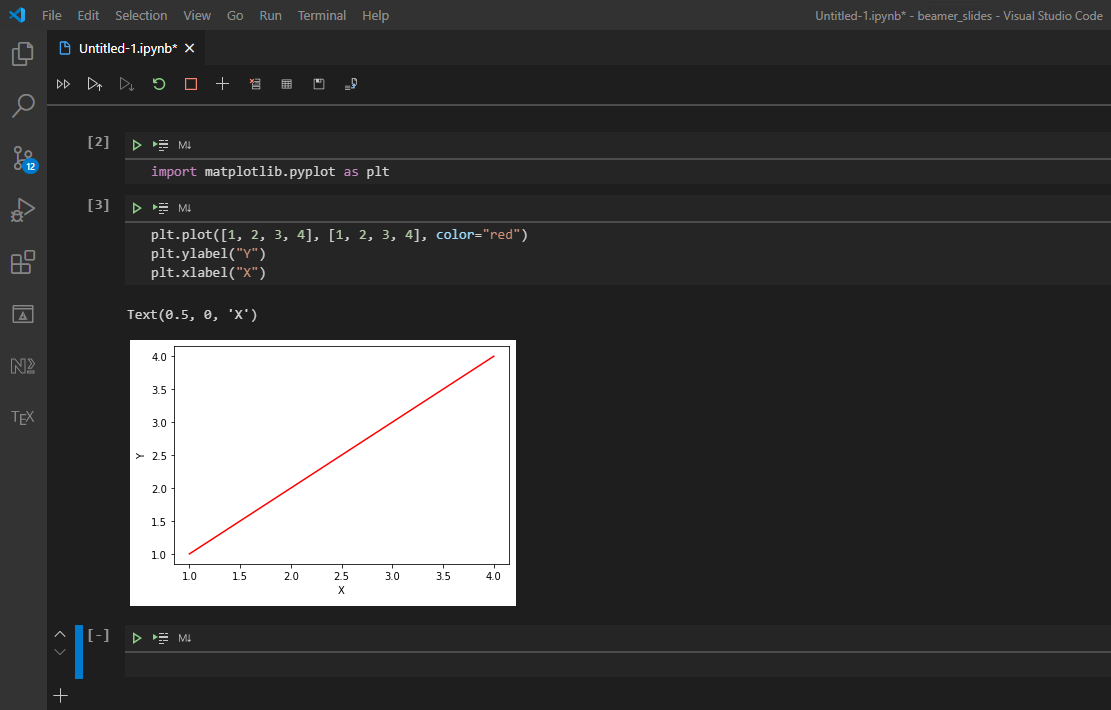
\includegraphics[width=0.9\textwidth]{screenshots/vsc-1.png}
    \end{center}				
\end{frame}

\begin{frame}[fragile]
	\frametitle{Matplotlib from the Command Line}
    \begin{itemize}
      \item Create a file \keyword{my-first-plot.py}
    \end{itemize}
    \begin{block}{File: my-first-plot.py}
    \begin{lstlisting}[language=Python]
    import matplotlib.pyplot as plt
    plt.plot([1,2,3,4], [1, 4, 9, 16], color="red")
    plt.show()
    \end{lstlisting}      
		\end{block}		
    \begin{itemize}
      \item Run the python script \keyword{python ./my-first-plot.py}
    \end{itemize}			
    \begin{center}
      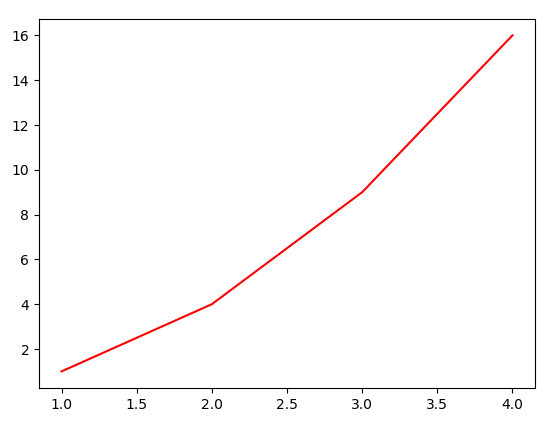
\includegraphics[width=0.25\textwidth]{screenshots/plt-2.png}
    \end{center}						
\end{frame}

\begin{frame}[fragile]
   \vspace{-1cm}
    \begin{center}
      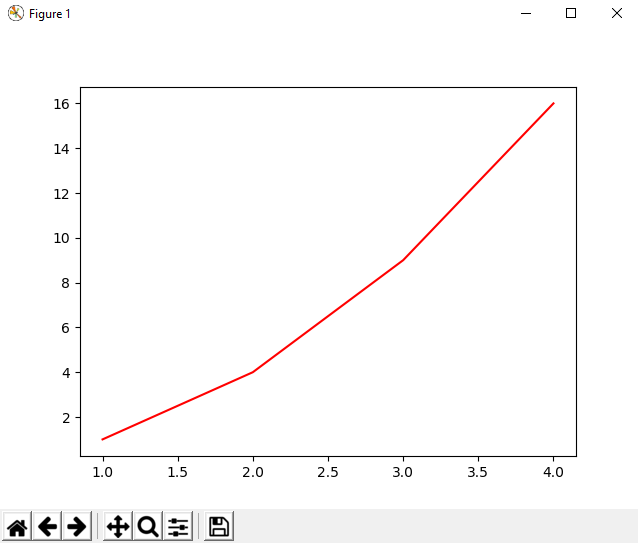
\includegraphics[width=0.7\textwidth]{screenshots/plt-1.png}
    \end{center}						
\end{frame}

\begin{frame}[fragile]
	\frametitle{Components of a Matplotlib Plot}
    \begin{itemize}
      \item \keyword{Figure (object)}: The top-level component, the whole window/container of the plot
      \item \keyword{Axes}: The area containing the plot data, labels, axis ticks, etc. 
      \item The term \keyword{Subplot} in Matplotlib is in most cases the same as \keyword{Axes} 
      \item \keyword{XAxis} and \keyword{YAxis}: Are the corresponding parts of the \keyword{Axes} object
      \item Knowledge of these components makes it easier to add/change properties 
    \end{itemize}
\end{frame}

\begin{frame}[fragile]
   \vspace{-1cm}
    \begin{center}
      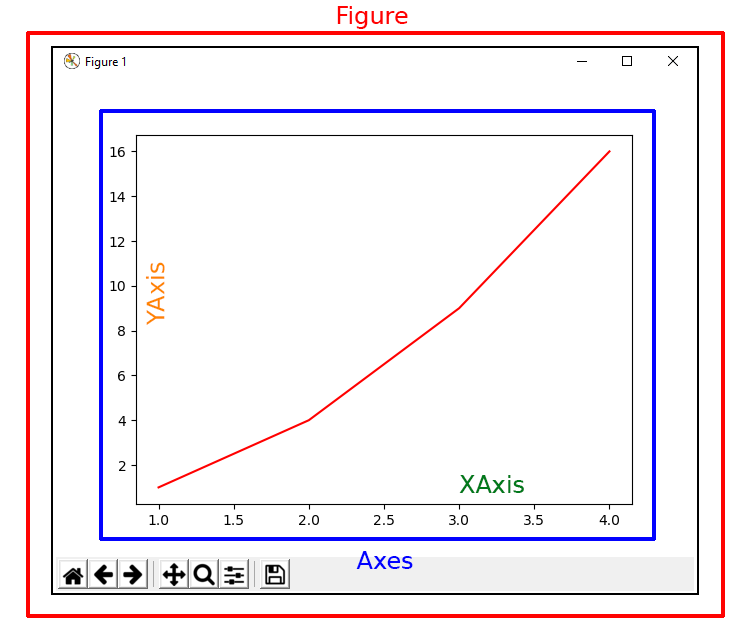
\includegraphics[width=0.7\textwidth]{screenshots/plt-3.png}
    \end{center}						
\end{frame}

\begin{frame}[fragile]
	\frametitle{Reading Data from a File}
    \begin{itemize}
      \item Create a file \keyword{my-second-plot.py}
    \end{itemize}
    \begin{block}{File: my-second-plot.py}
    \begin{lstlisting}[language=Python]
    import matplotlib.pyplot as plt
		import numpy as np
    data = np.loadtxt("data.txt")
    plt.plot(data[:,0], data[:,1], color="red")
		plt.show()
    \end{lstlisting}      
		\end{block}		
    \begin{itemize}
      \item Run the python script \keyword{python ./my-second-plot.py}
    \end{itemize}			
\end{frame}

\begin{frame}[fragile]
	\frametitle{Setting Axes Properties Explicitly}
    \begin{block}{File: plot-explicit.py}
    \begin{lstlisting}[language=Python]
import matplotlib.pyplot as plt
fig = plt.figure()
ax = fig.add_subplot(111)
ax.plot([1, 2, 3, 4], [10, 20, 25, 30], color='lightblue',
       linewidth=3)
ax.scatter([0.3, 3.8, 1.2, 2.5], [11, 25, 9, 26], 
          color='darkgreen', marker='^')
ax.set_xlim(0.5, 4.5)
plt.show()
    \end{lstlisting}      
		\end{block}		
\end{frame}

\begin{frame}[fragile]
	\frametitle{Setting Axes Properties Implicitly}
    \begin{block}{File: plot-implicit.py}
    \begin{lstlisting}[language=Python]
import matplotlib.pyplot as plt		
plt.plot([1, 2, 3, 4], [10, 20, 25, 30], color='lightblue',
        linewidth=3)
plt.scatter([0.3, 3.8, 1.2, 2.5], [11, 25, 9, 26], 
           color='darkgreen', marker='^')
plt.xlim(0.5, 4.5)
plt.show()
    \end{lstlisting}      
		\end{block}
    \begin{itemize}
      \item \keyword{Axes} functions/methods are called "behind the scenes"
      \item If multiple axes/subplots are present then use Axes object directly			
    \end{itemize}		
\end{frame}

\begin{frame}[fragile]
   \vspace{-1cm}
    \begin{center}
      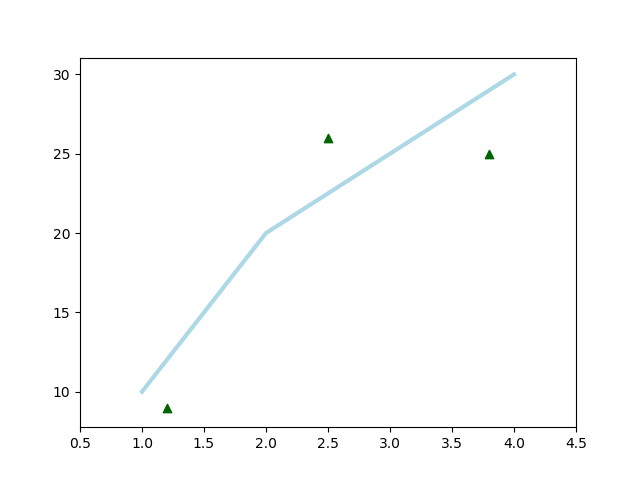
\includegraphics[width=0.7\textwidth]{screenshots/fig-ex-1.png}
    \end{center}						
\end{frame}

\begin{frame}[fragile]
	\frametitle{Using the API Documentation}
    \begin{itemize}
      \item https://matplotlib.org/contents.html
    \end{itemize}			
   \vspace{2cm}			
    \begin{center}
      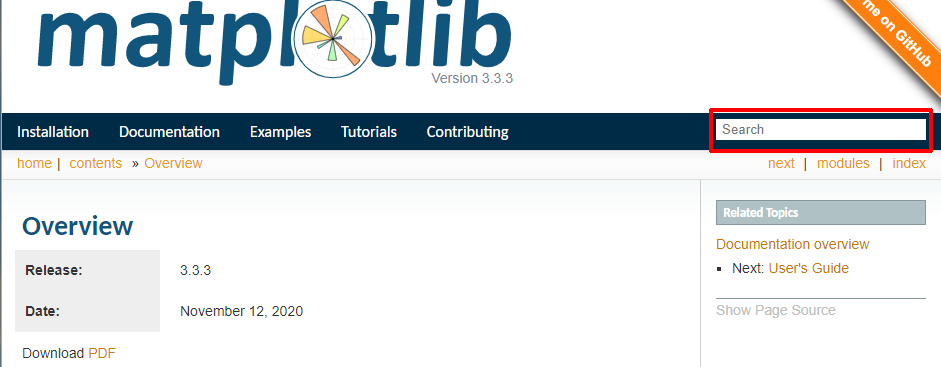
\includegraphics[width=0.8\textwidth]{screenshots/manual-api.png}
    \end{center}						
\end{frame}

\begin{frame}[fragile]
	\frametitle{Plot Customization}
    \begin{block}{File: plot-custom-1.py}
    \begin{lstlisting}[language=Python]
X = np.linspace(-np.pi, np.pi, 256, endpoint=True)
Cos, Sin = np.cos(X), np.sin(X)
plt.plot(X, Cos, color="blue", linewidth=2.5, linestyle="-", label="Kosinus")
plt.plot(X, Sin, color="red",  linewidth=2.5, linestyle="--", label="Sinus")
# Gitter 
plt.grid()
# Titel
plt.title("Sinus und Kosinus",loc="center")
# Legende
plt.legend(loc="best", frameon=False)
    \end{lstlisting}      
		\end{block}
\end{frame}

\begin{frame}[fragile]
   \vspace{-1cm}
    \begin{center}
      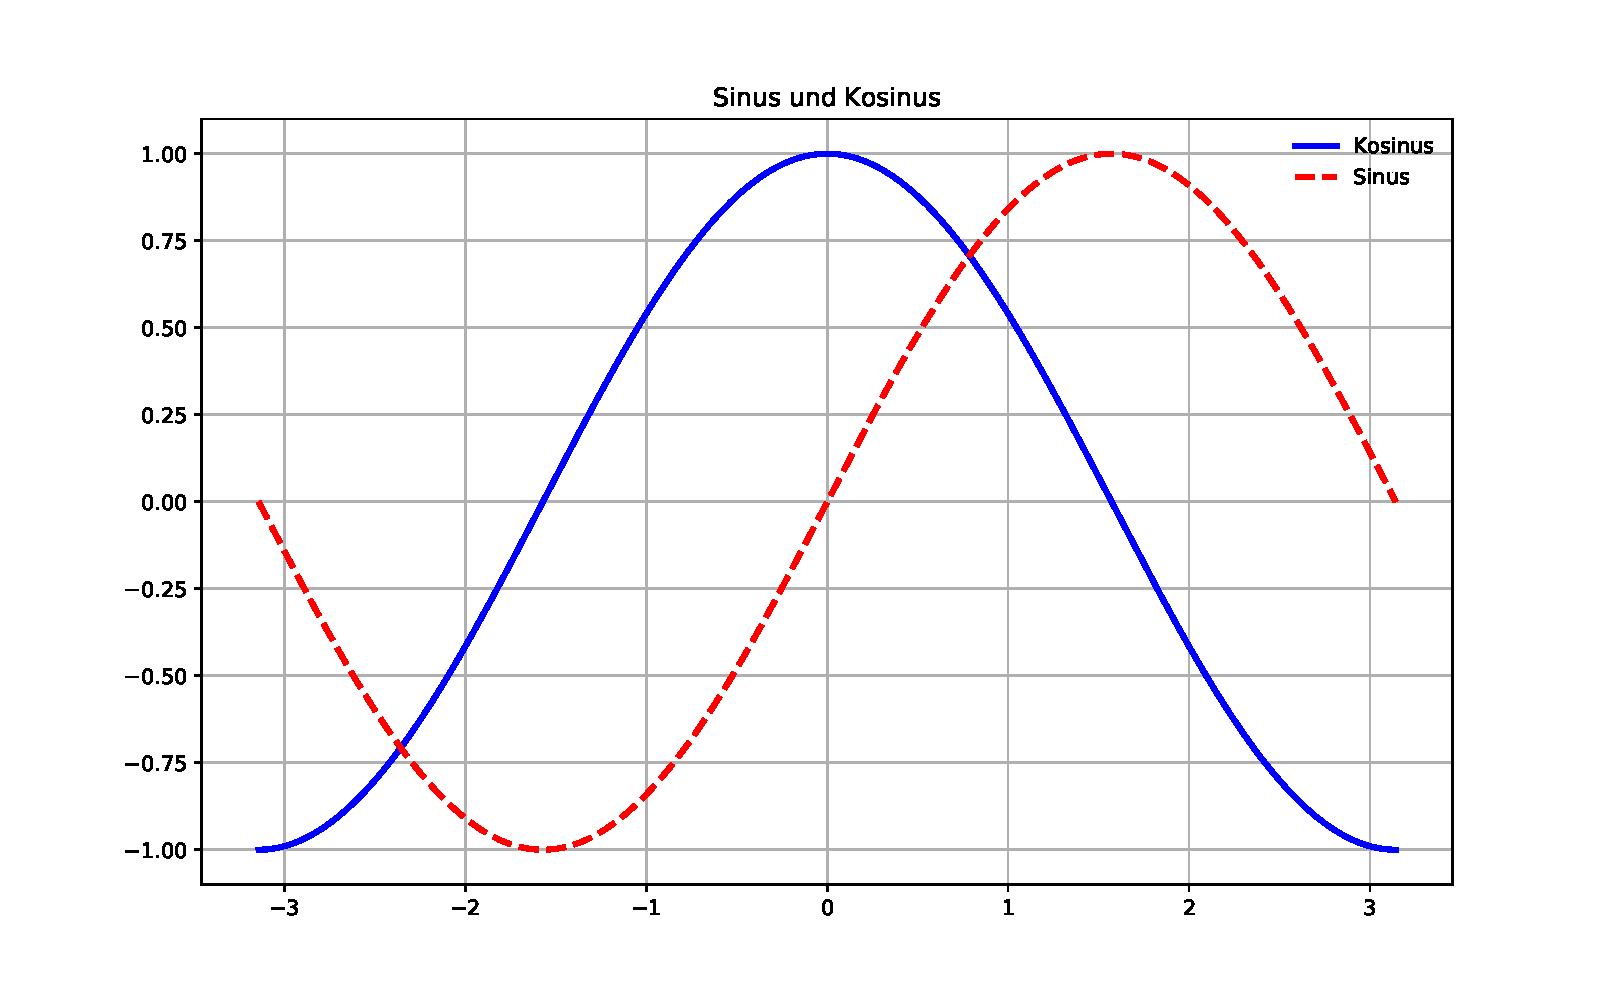
\includegraphics[width=0.9\textwidth]{screenshots/plt-4.pdf}
    \end{center}						
\end{frame}

\begin{frame}[fragile]
	\frametitle{Plot Customization II}
    \begin{block}{File:  plot-custom-1.py continued}
    \begin{lstlisting}[language=Python]
# Legende
plt.legend(loc="best", frameon=True)
plt.xticks([-np.pi, -np.pi/2, 0, np.pi/2, np.pi],
       [r'$-\pi$', r'$-\pi/2$', r'$0$', r'$+\pi/2$', r'$+\pi$'])
plt.yticks([-1, 0, +1],
       [r'$-1$', r'$0$', r'$+1$'])
    \end{lstlisting}      
		\end{block}
    \begin{itemize}
      \item r'text' is a raw string
      \item Inside a raw string \$ can be used to enter latex equations
    \end{itemize}					
\end{frame}

\begin{frame}[fragile]
   \vspace{-1cm}
    \begin{center}
      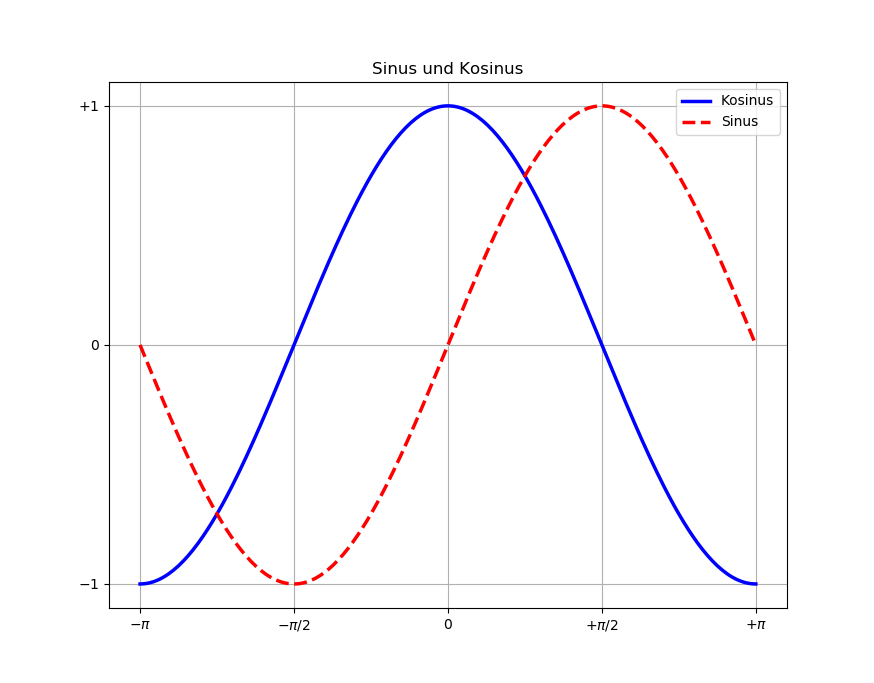
\includegraphics[width=0.85\textwidth]{screenshots/plt-5.png}
    \end{center}						
\end{frame}

\begin{frame}[fragile]
	\frametitle{Plot Customization III}
    \begin{itemize}
      \item Highlight data points using the \keyword{annotate} function
      \item Configure the \keyword{spines} of the subplot
      \item \keyword{Spines} are the 4 lines bordering the plot area 
      \item Stored in python dictionary with keys: 'top', 'left', 'bottom', 'right'
      \item Text labels usually have a fontsize	property that can be adjusted		
    \end{itemize}					
\end{frame}

\begin{frame}[fragile]
   \vspace{-1cm}
    \begin{center}
      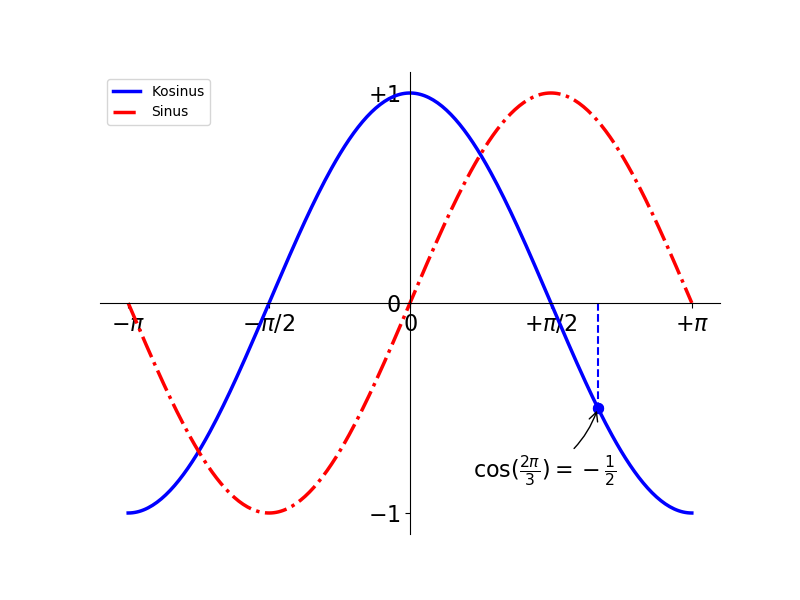
\includegraphics[width=0.85\textwidth]{screenshots/plt-6.png}
    \end{center}						
\end{frame}

\begin{frame}[fragile]
	\frametitle{Subplots and Plot Types}
    \begin{itemize}
      \item Subplots can be grouped in a grid of plots
    \begin{block}{Create subplot with two rows and columns}
    \begin{lstlisting}[language=Python]
			fig, axes = plt.subplots(nrows=2, ncols=2)		
			# Set title for a single subplot
			axes[1,0].set_title('Title for 2nd row 1st column')
    \end{lstlisting}      
		\end{block}
      \item Large variety of plot types as in Matlab
      \item Bar plot, pie plot, contour plot, histograms, stream plots, 3D plots, $\ldots$ 
			\item \url{https://matplotlib.org/tutorials/introductory/sample_plots.html}
    \end{itemize}					
\end{frame}

\begin{frame}[fragile]
   \vspace{-1cm}
    \begin{center}
      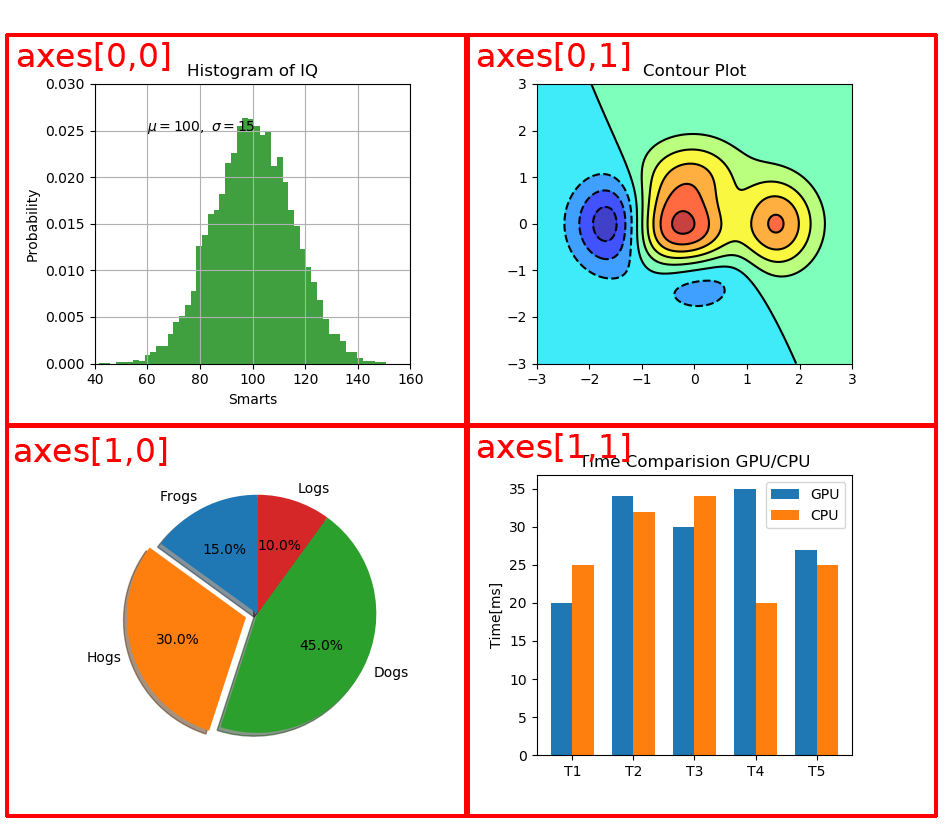
\includegraphics[width=0.7\textwidth]{screenshots/plt-8.png}
    \end{center}						
\end{frame}

\begin{frame}[fragile]
	\frametitle{Saving Plots to a File from a Script}
    \begin{itemize}
      \item Subplots can be grouped in a grid of plots			
    \begin{block}{plot-savefig.py}
    \begin{lstlisting}[language=Python]			
			fig, ax = plt.subplots()			
			ax.plot(t, s)
			ax.set(xlabel='time (s)', ylabel='voltage (mV)',
						 title='A Simple Plot')
			ax.grid()
			fig.savefig("test.pdf")			
    \end{lstlisting}      
		\end{block}						
    \end{itemize}					
\end{frame}

\begin{frame}[fragile]
	\frametitle{Using Matplotlib on a Cluster without Graphical Interface}
    \begin{itemize}
      \item Design your desired postprocessing plot in i.e. Jupyter notebook
      \item Save your python code to a script, eventually add file handling/manipulation code			
      \item Add code to save your plot to a file				
      \item Transfer the script to the compute cluster						
      \item Execute script on the cluster, transfer the resulting file to local computer									
    \end{itemize}					
\end{frame}